\chapter{Experiment No.2: The Haynes and Shockley-Experiment}
\section{Description}
\subsection*{Experimental Setup}
In this experiment we should determine the behavior of charge carriers in materials. Our material was Germanium. First we need free charge carrier to observe. To get them we use a laser to geht electron (our charge carrier) from the valence band to the conduction band. The laser is activated in short periodic impulses so we get little cluster of electrons. A voltage applied on the Ge accelerate our electron clusters in its electric field. To detect the cluster we using a detector so we could visualize the signal on an oscilloscope. Impuls and measuring happens 30 times per second (30Hz).
\begin{figure}[h]
\begin{center}
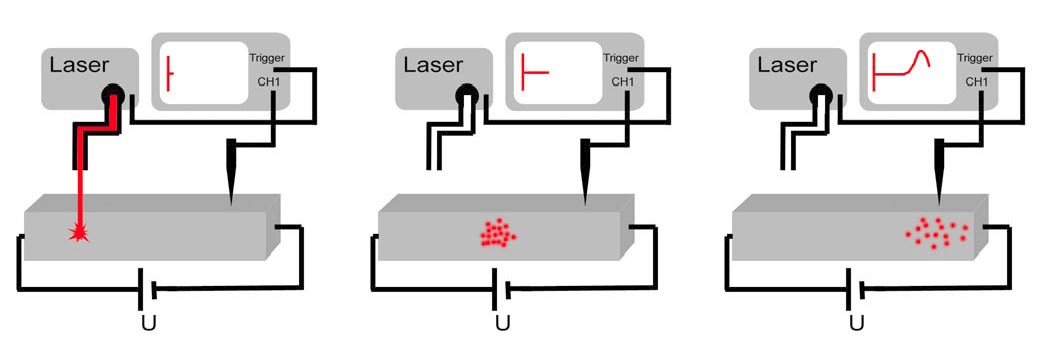
\includegraphics[scale=0.5]{Bilder/aufbau_teil2}
\caption{Experimental setup. Source:[Ver] }
\label{fig:aufbau2}
\end{center}
\end{figure}
\section{Analysis}
To get the mean time $\mathit{\tau}$, the mean free path and the mass diffusivity $\mathit{D_{e}}$ of the electrons in our p-Ge, we fitted normal distribution on the measured electron clusters of the oscilloscope. The normal distribution is given as:\\
\begin{center}
$\mathit{c(x)=A\frac{1}{\sqrt{2\pi \sigma^2}}}\exp\left(-\dfrac{(x-x_{c})^2}{2\sigma^2}\right)$
\end{center}
$\mathit{A}$,$\mathit{x_{c}}$ and $\mathit{\rho}$ are the known parameter of a normal distribution.\\
\\
The differential equation of an electron in a p-doped semiconductor is given as followed:\\
\begin{center}
$\mathit{c(t,x)=C\exp(-t/\tau_{n})\frac{1}{\sqrt{4\pi D_{e}t}} \exp\left(-\dfrac{(x-\mu_{n}Et)^2}{4D_{e}t}\right)}$
\end{center}
$\mathit{C}$ : Constant\\
$\mathit{\tau_{n}}$ : Mean time\\
$\mathit{D_{n}}$: Mass diffusivity\\
$\mathit{\mu_{n}}$ : Mobility of the free electrons\\
$\mathit{E}$ : Electrical field strength\\

Compare now the parameter of these two functions, it's easy to find the followed relationships:
\begin{tabbing}
$\mathit{x_{c}(t)=\mu_{n}Et}$,\\
$\mathit{A(t)=C \exp(-t/\tau_{n})}$,\\
$\mathit{\sigma(t)=\sqrt{2D_{n}t}}$,\\
\end{tabbing}
To get $\mathit{\mu_{n}}$, $\mathit{\tau_{n}}$ and $\mathit{D_{n}}$ we can fit these relations and get them from the parameter of the fits.
This approach works for the first series of measurements as well as for the second. 
\newpage
\subsection*{1. Measurements}
We put the normal distribution in the appendix, because of the big number of fits. Out of that fit we got our parameter for the following fits.
To get the mobility $\mathit{\mu_{n}}$ we can use the linear relation with the distance between laser and detector on the Ge.
\begin{figure}[h]
\begin{center}
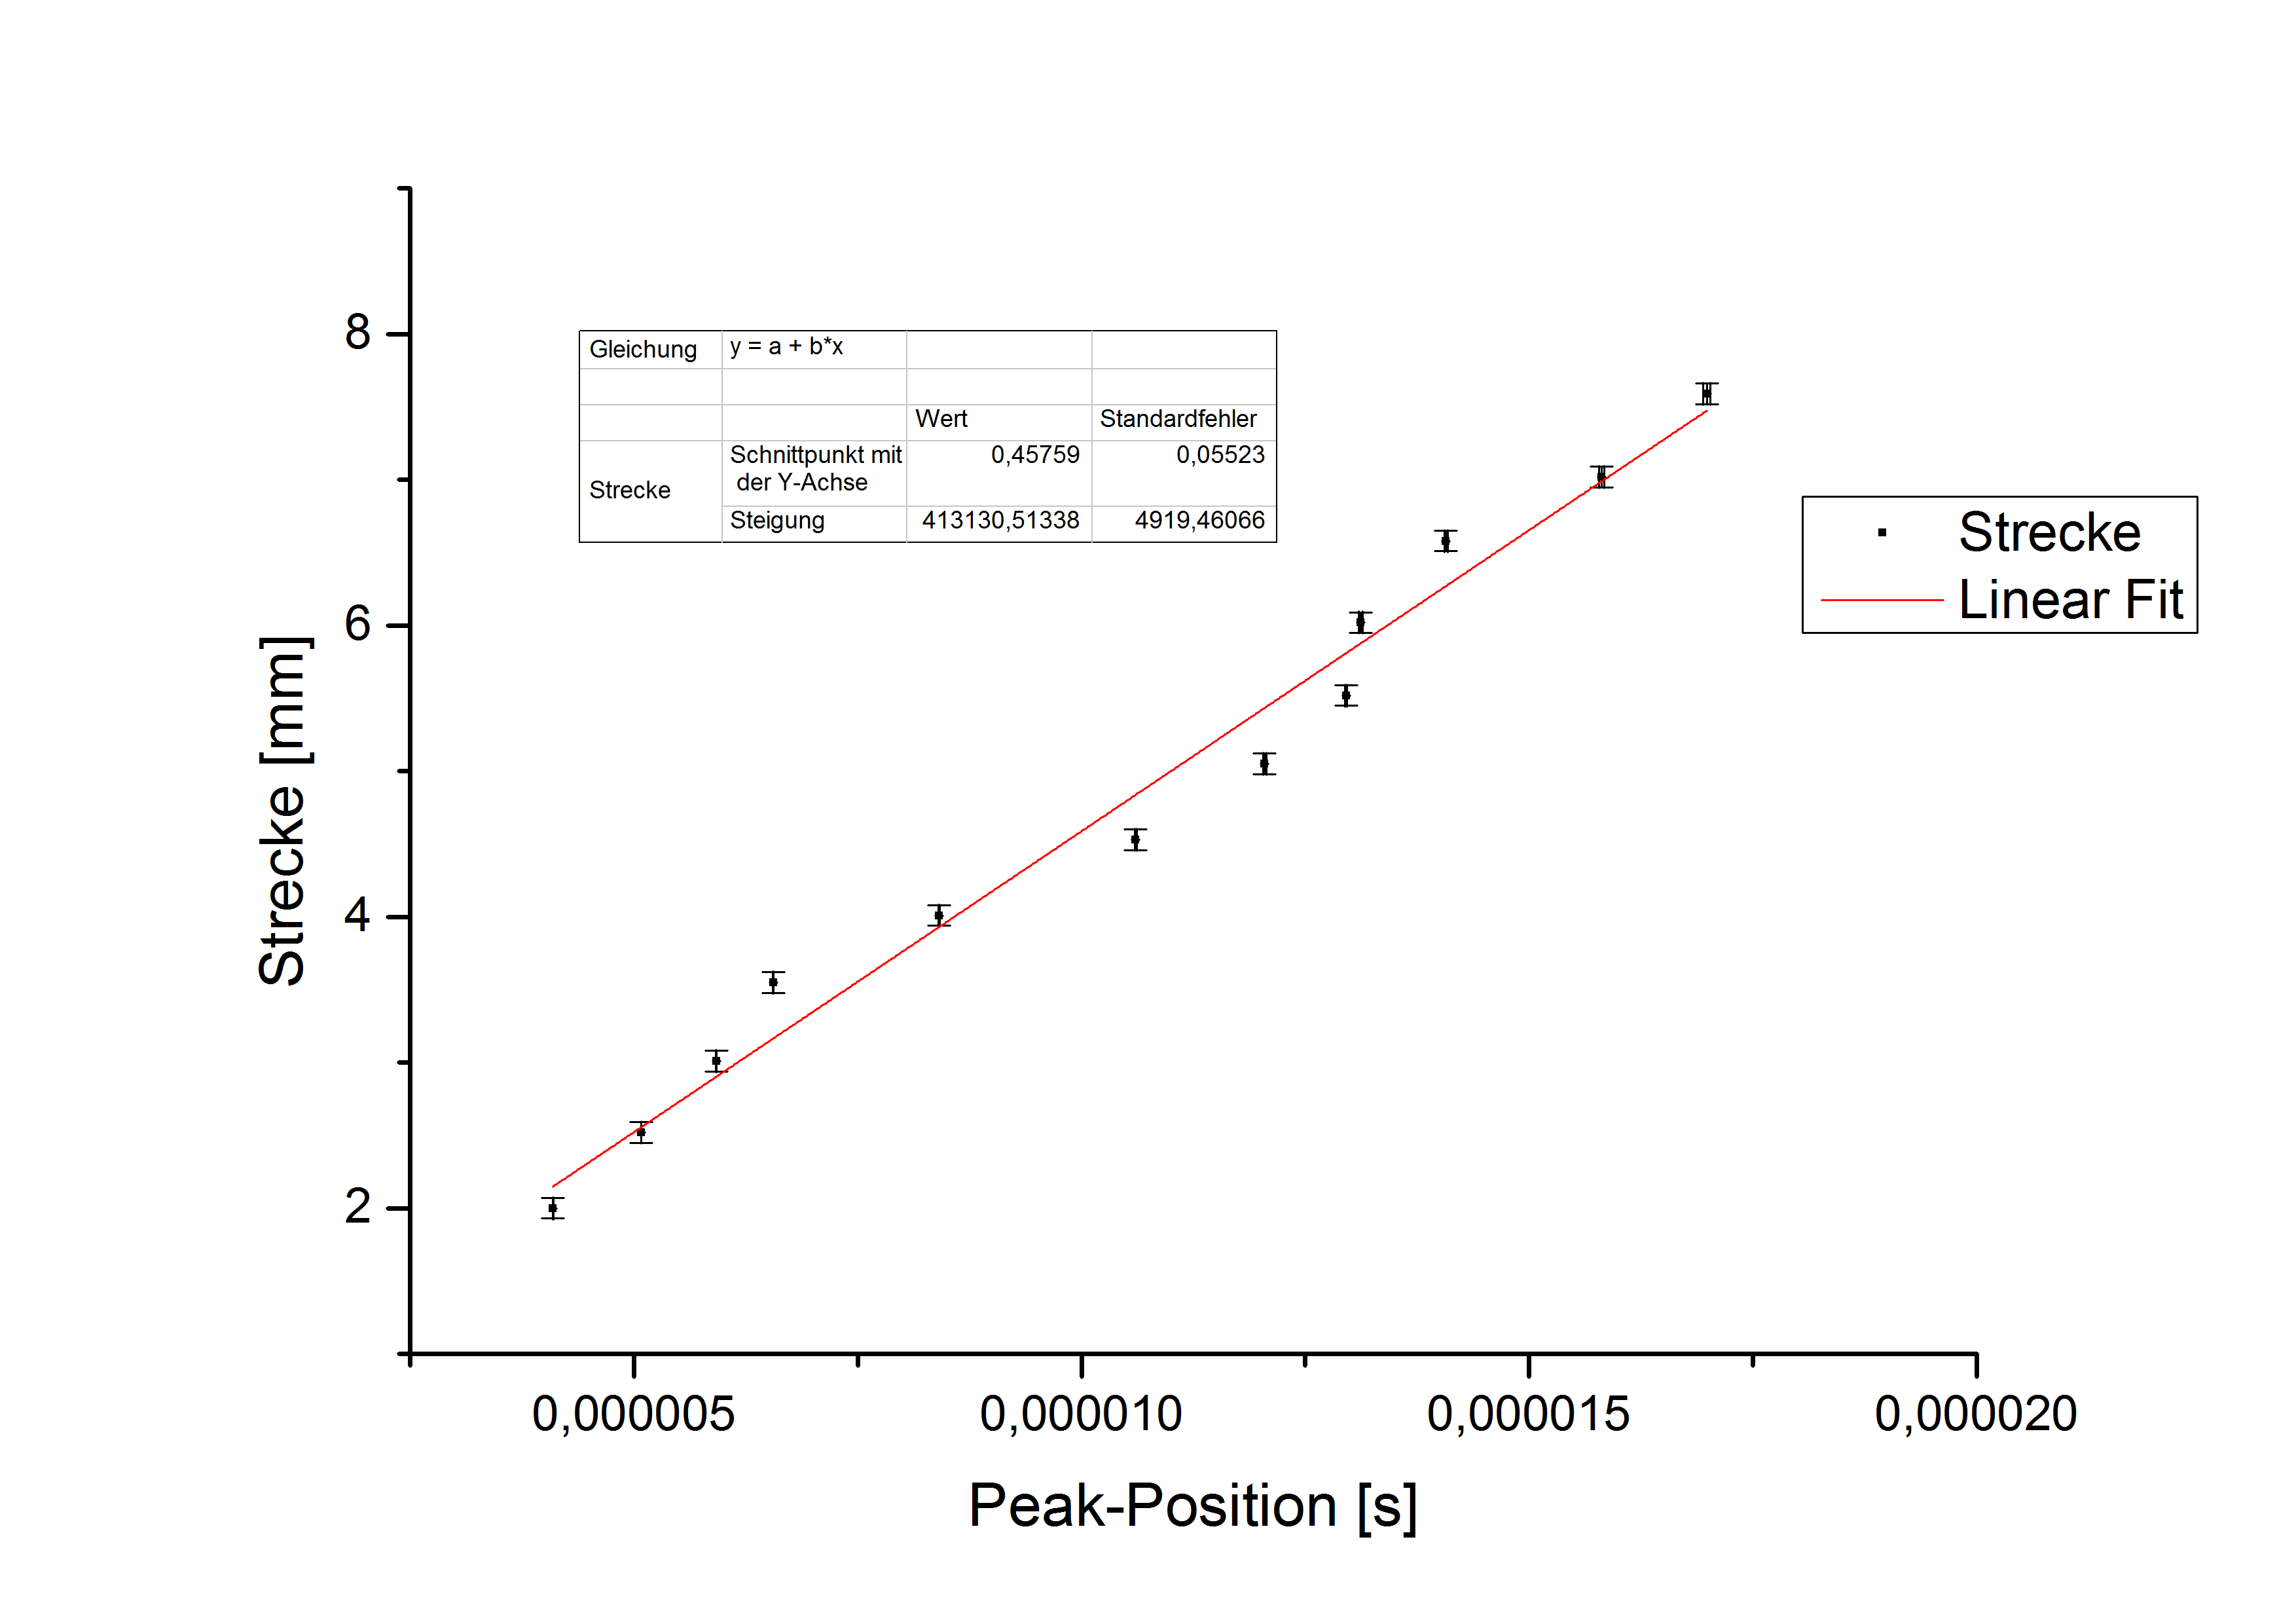
\includegraphics[scale=0.5]{Bilder/t2_1_my}
\caption{Linear relation of the distance to $\mathit{\mu_{n}}$. }
\label{fig:1my}
\end{center}
\end{figure}
The electric field $\mathit{E=(1.70\pm0.04)\frac{V}{mm}}$. It is easy to see that out $\mathit{x_{c}(t)=\mu_{n}Et}$ the $\mathit{\mu_{n}E}$ corresponds to the pitch $\mathit{b}$, so $\mathit{\mu_{n}=b/E}$ and $\mathit{s_{\mu_{n}}=\sqrt{(\frac{s_{b}}{E})^2+(-\frac{b}{E^2}s_{E})^2}}$.
\newpage
The mean lifetime $\mathit{\tau}$ is directly calculated and shown as a parameter of the fit.
\begin{figure}[h]
\begin{center}
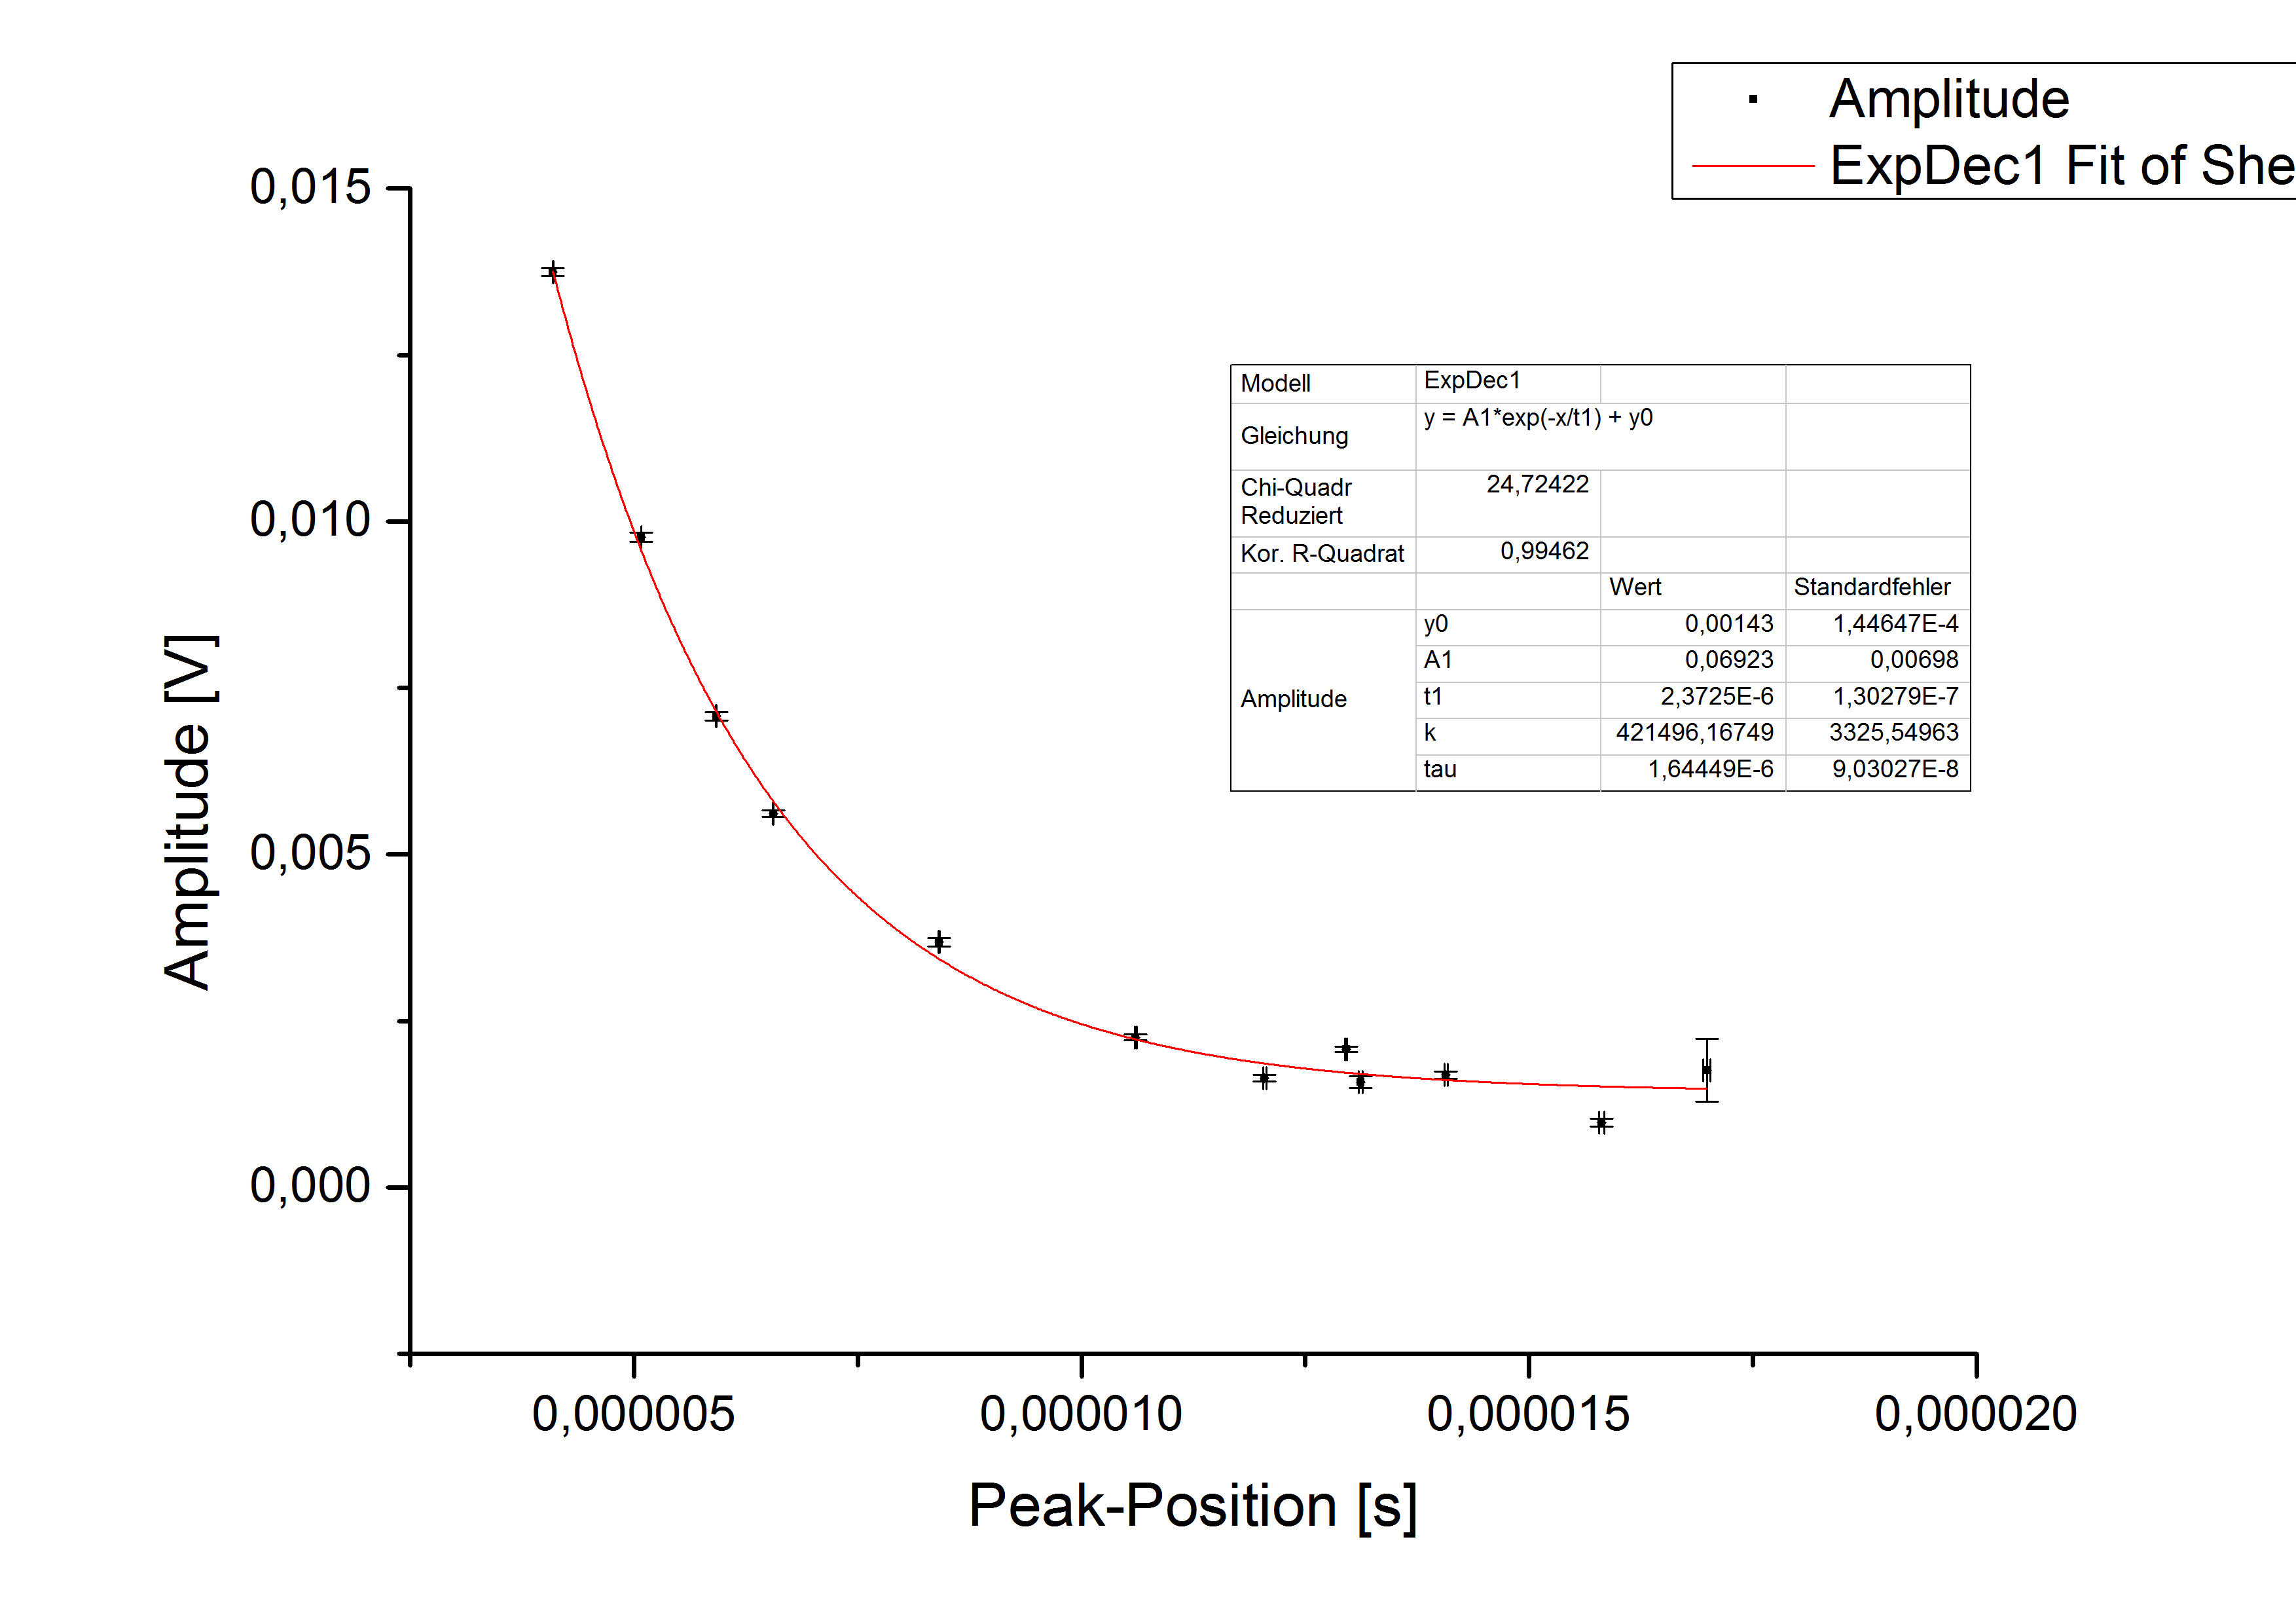
\includegraphics[scale=0.5]{Bilder/t2_1_tau}
\caption{Exponential decay as fit of the amplitude, to get $\mathit{\tau_{n}}$. }
\label{fig:1tau}
\end{center}
\end{figure}
\newpage
The square-root-function gives us the mass diffusivity $\mathit{D_{e}}$:
\begin{figure}[h]
\begin{center}
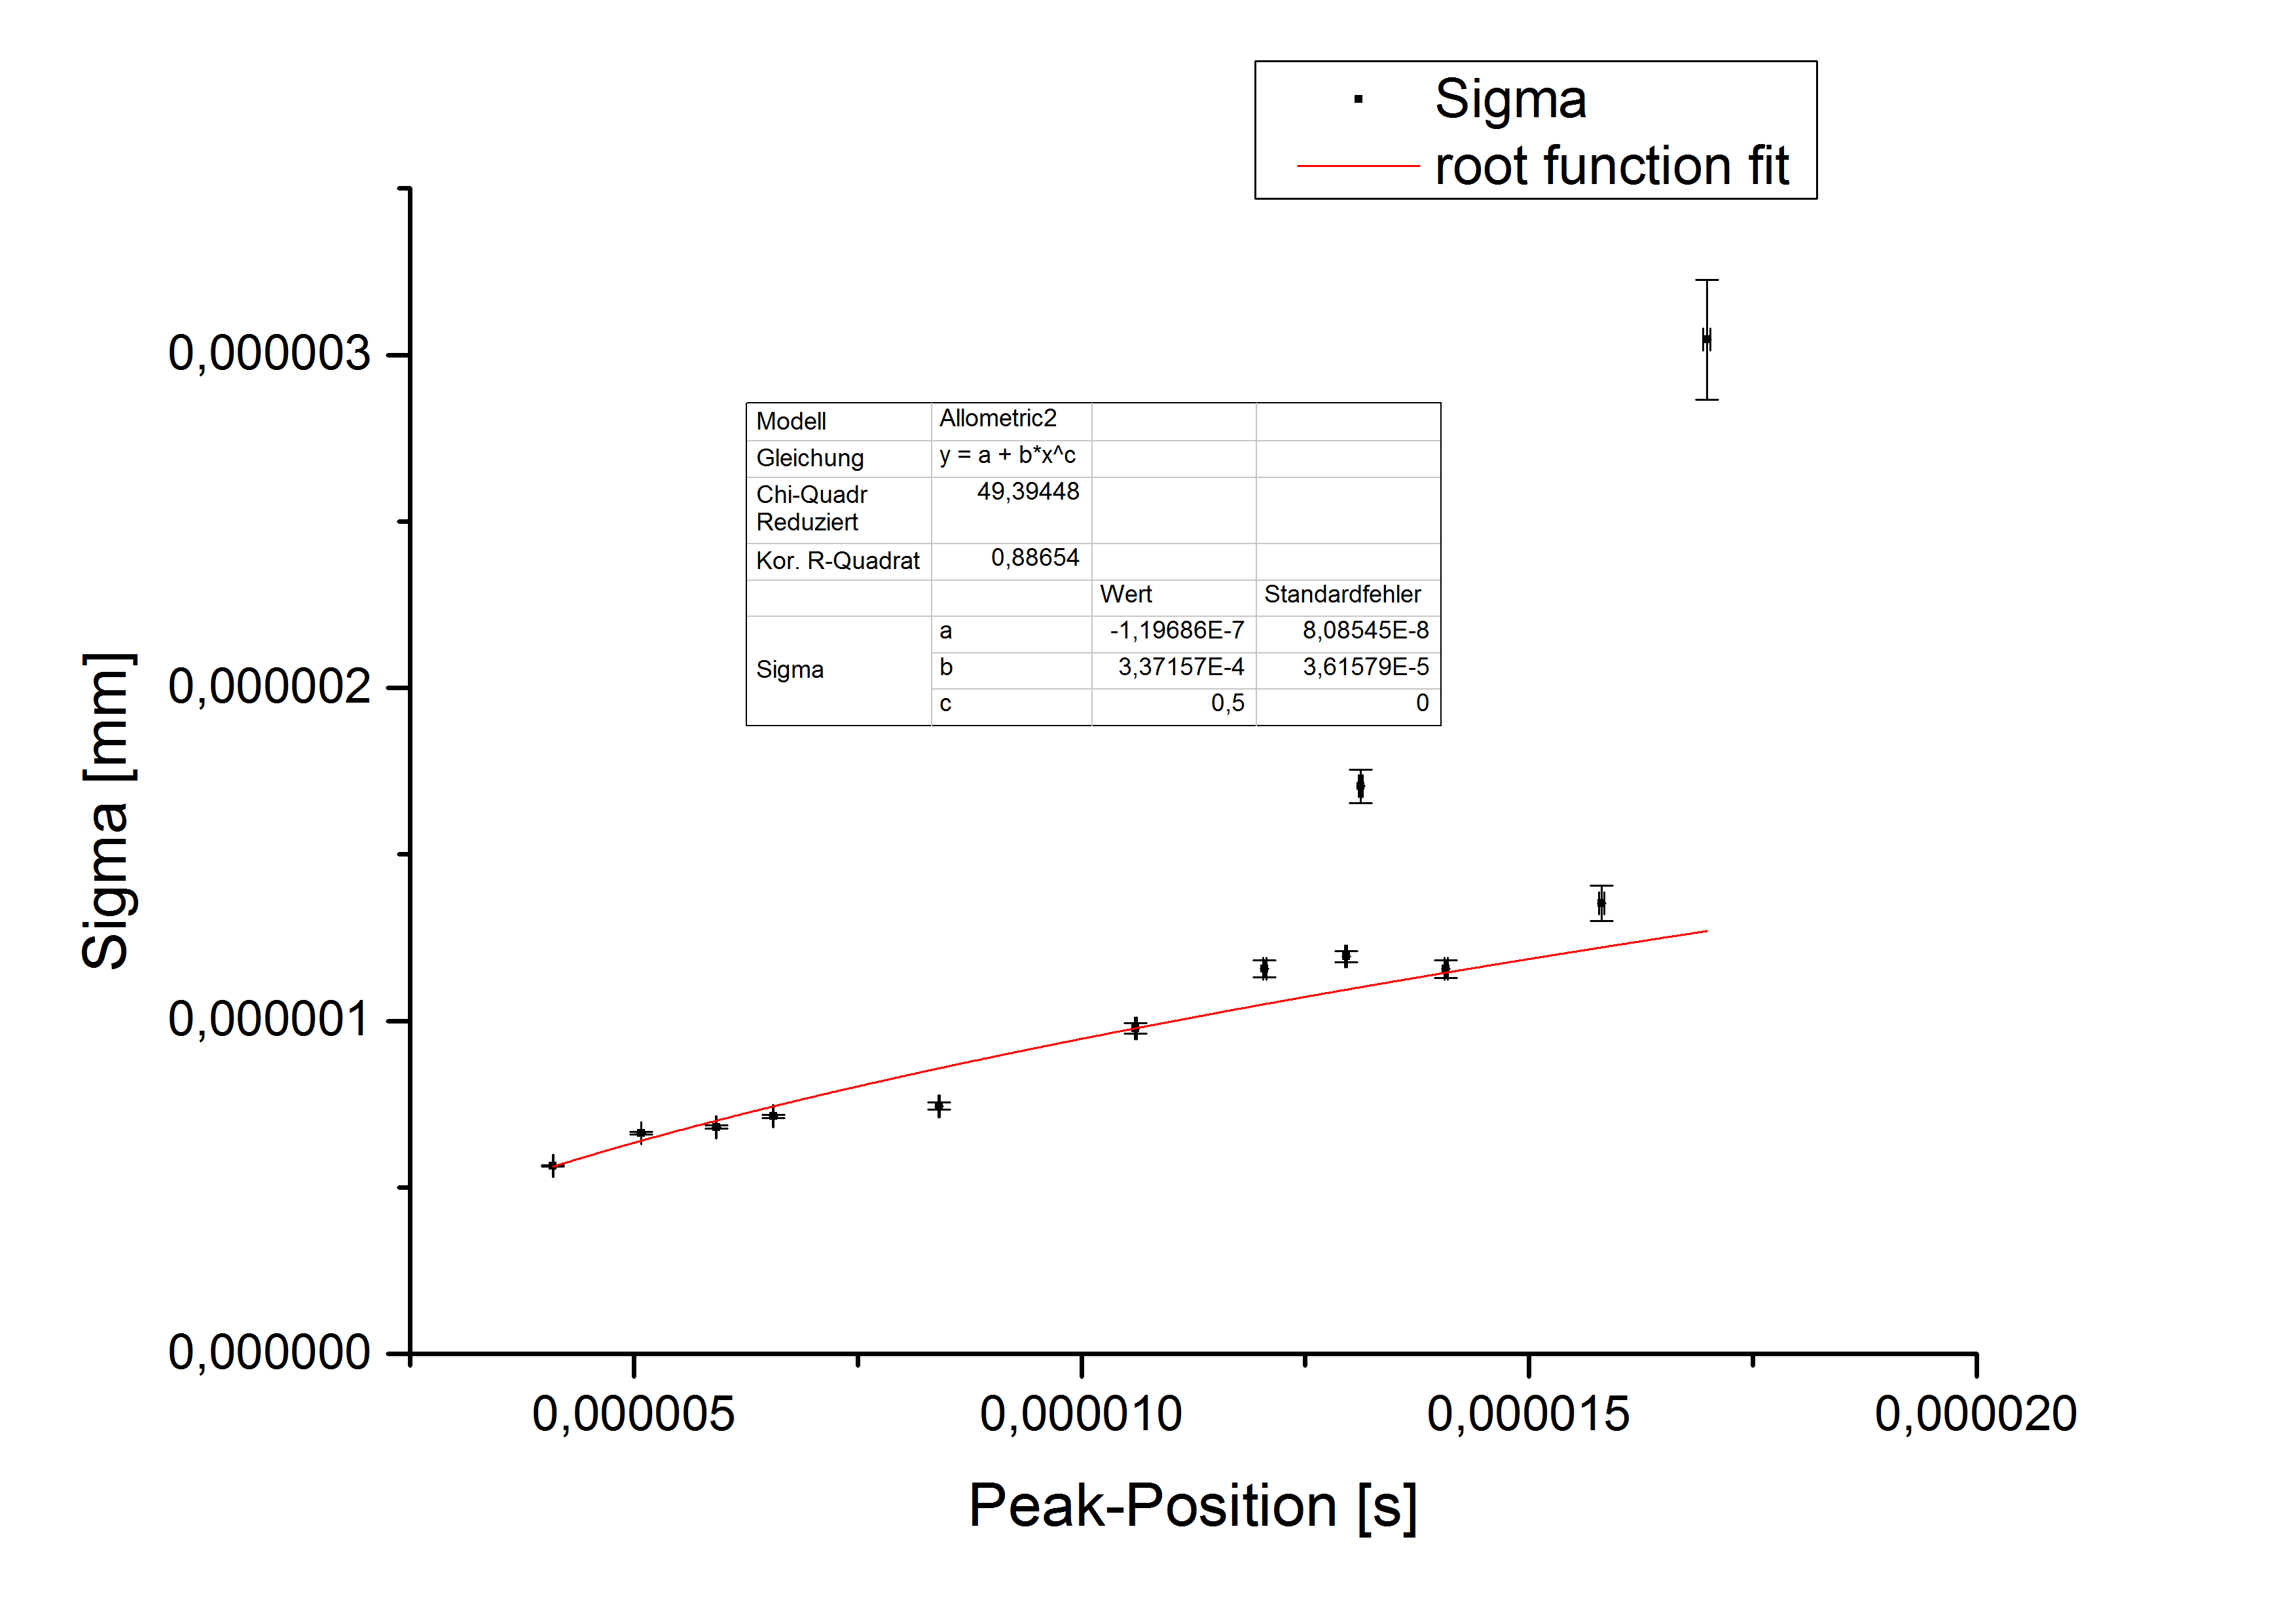
\includegraphics[scale=0.5]{Bilder/t2_1_sigma}
\caption{Square root function as fit of the sigma, to get $\mathit{D_{e}}$. }
\label{fig:1sigma}
\end{center}
\end{figure}\\
Easy to see that $\mathit{b^2= 2 D_{e}}$, so we get:\\
$\mathit{D_{e}=\frac{b^2}{2}}$ and \\
$\mathit{s_{D_{e}}=b\cdot s_{b}}$.\\
\\
So our results from the first series of measurements is:\\

$\mathit{\mu_{n}=(2420\pm70)\frac{cm^{2}}{Vs}}$\\

$\mathit{\tau_{n}=(2.4\pm0.1)\cdot10^{-6}s}$\\

$\mathit{D_{e}=(5\pm1)\cdot10^{-8}\frac{mm^{2}}{s}}$
\newpage
\subsection*{2. Measurements}
At the variation of the charge, we had $\mathit{x_{c}(t)=\mu_{n}\frac{U}{l}t}$ an form it to $\mathit{U(t)=\frac{x_{c} \cdot l}{\mu_{n}}\frac{1}{t}}$, at which $\mathit{x_{c}(t)=const}$ an $\mathit{l}$ is the length of the Ge-pad. The $\mathit{1/x}$-function fit gives us:\\
\begin{figure}[h]
\begin{center}
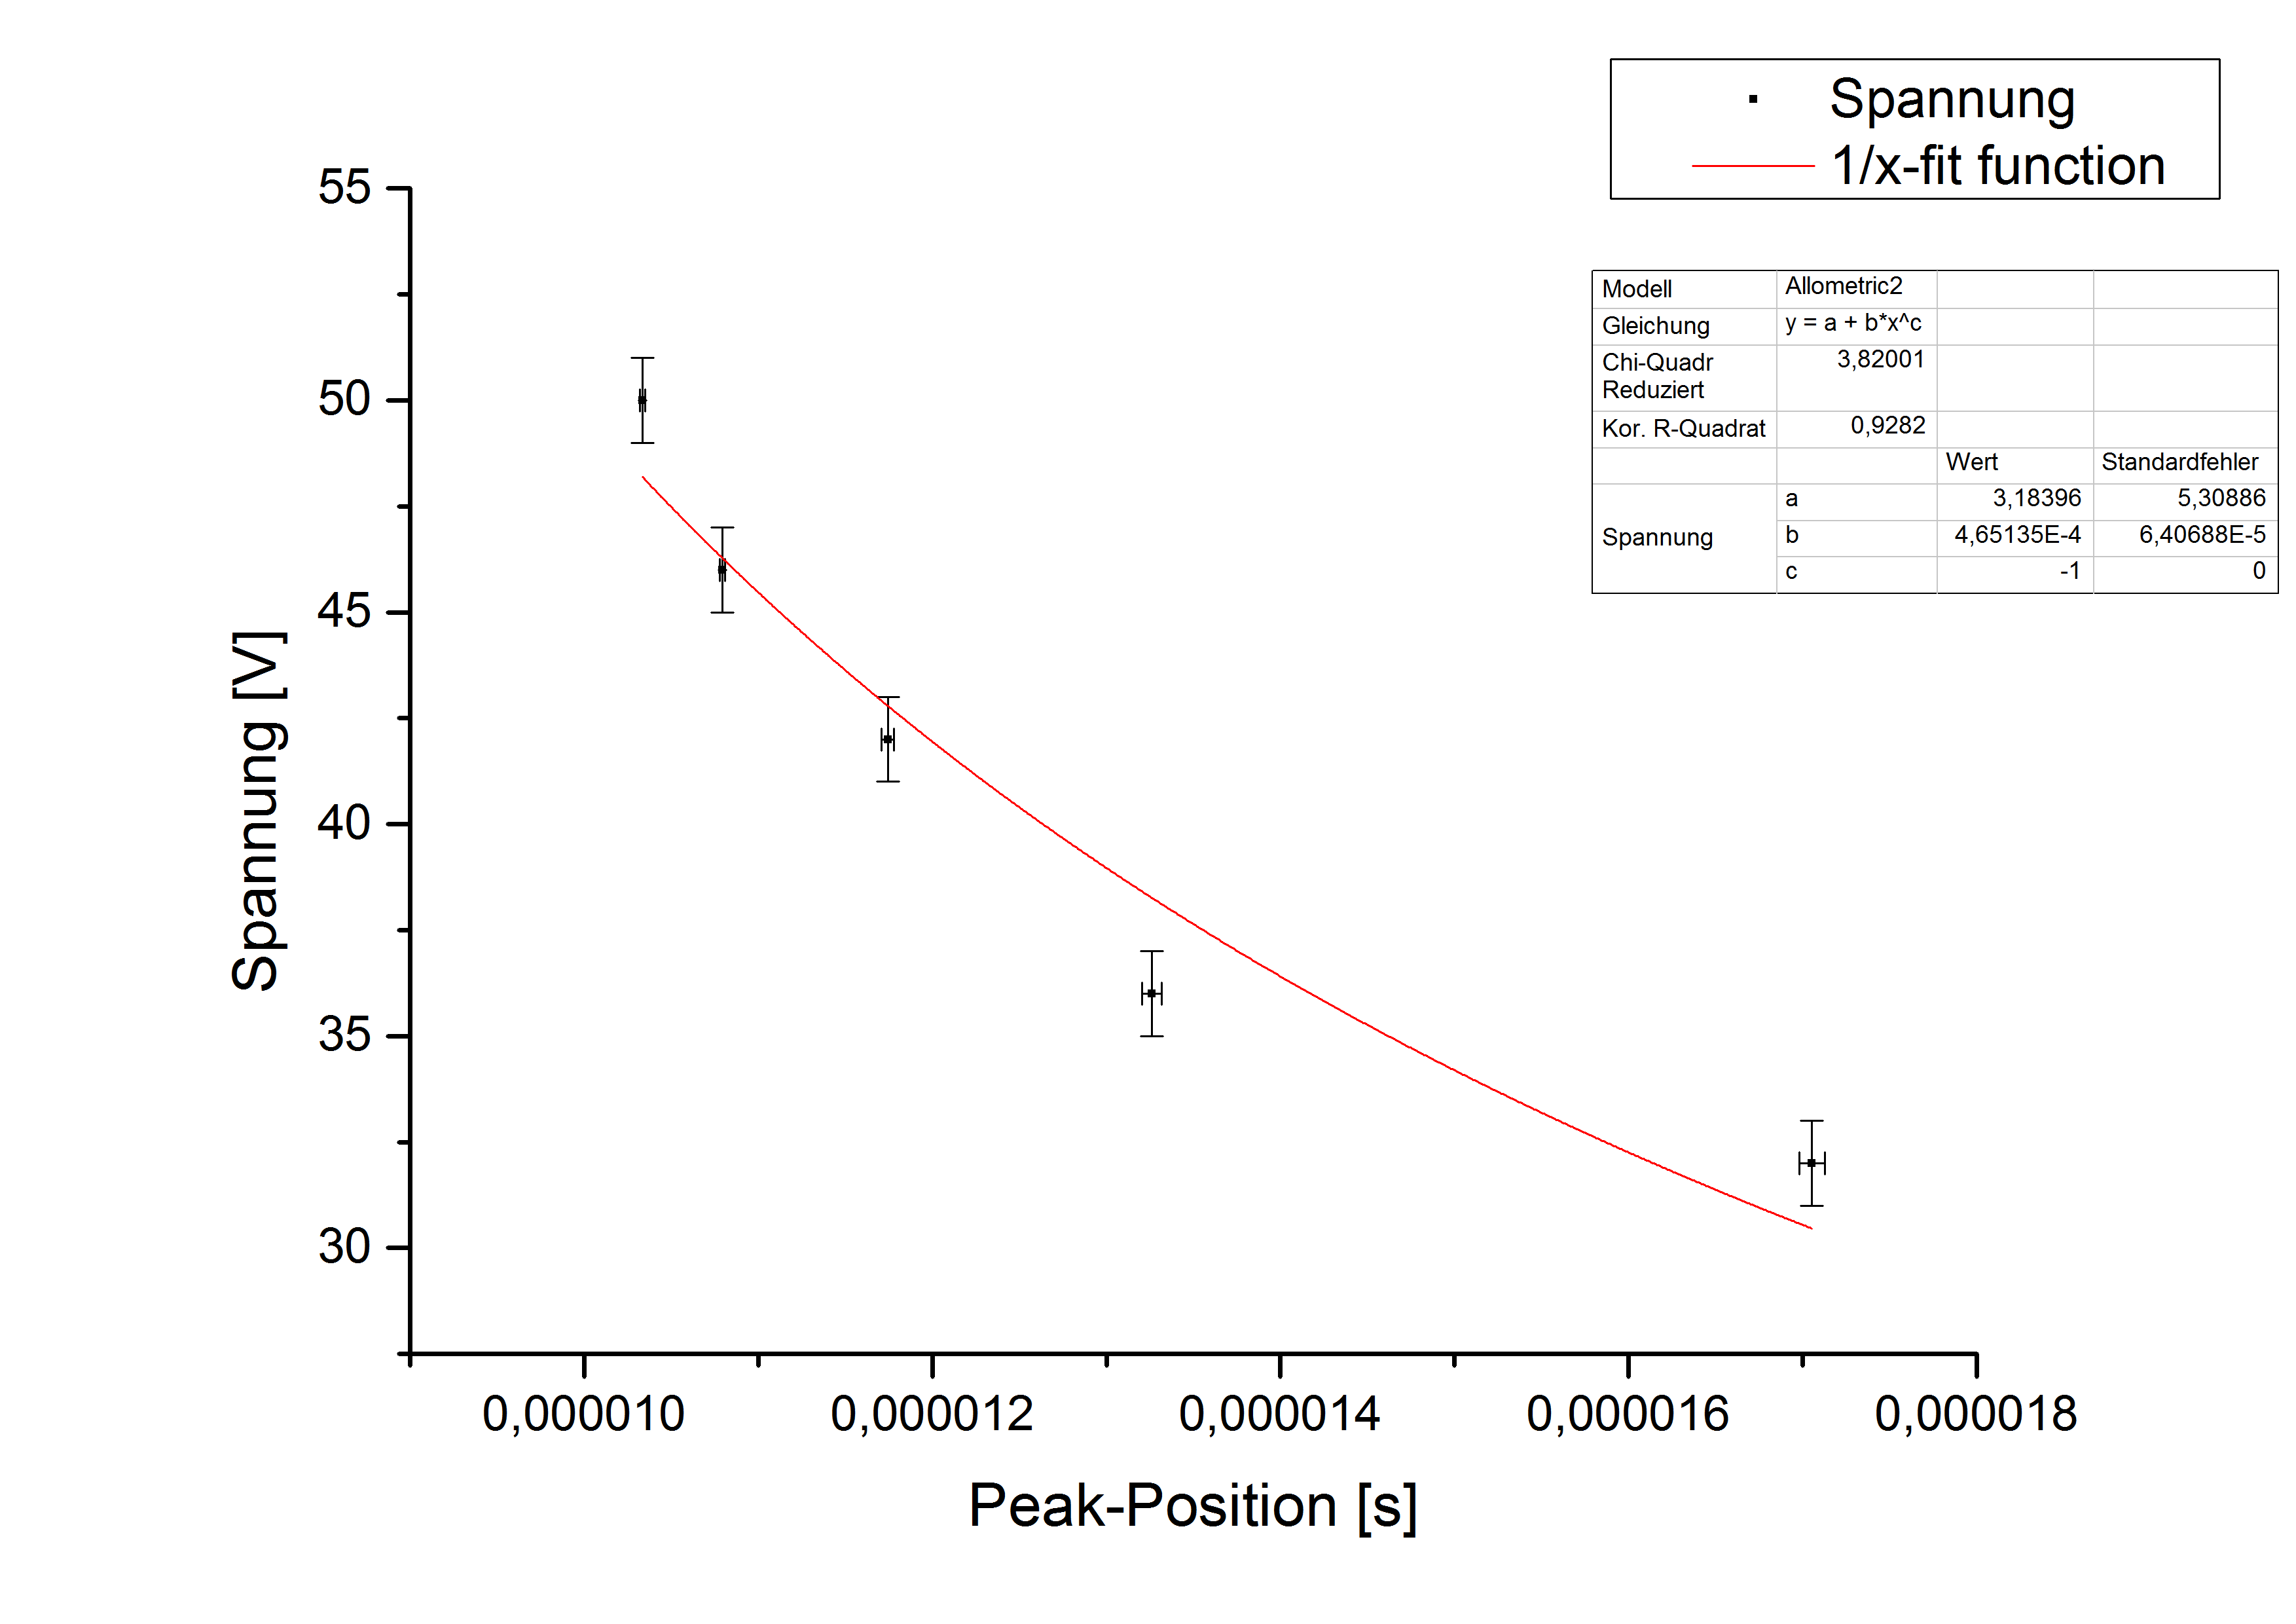
\includegraphics[scale=0.5]{Bilder/t2_2_my}
\caption{$\mathit{1/x}$-function fit of the voltage, to get $\mathit{\mu_{n}}$. }
\label{fig:2my}
\end{center}
\end{figure}\\
With the parameter $\mathit{b}$ is $\mathit{\mu_{n}=\frac{x_{c} \cdot l}{b}}$ and $\mathit{s_{\mu_{n}}=\sqrt{(\frac{l}{b}\cdot s_{x_{c}})^2+(\frac{x_{c}}{b}\cdot s_{l})^2+(\frac{x_{c} \cdot l}{b^2}\cdot s_{b})^2}}$ we can calculate $\mathit{\mu_{n}}$.
\newpage
$\mathit{\tau}$ can be read out of the fit parameters.
\begin{figure}[h]
\begin{center}
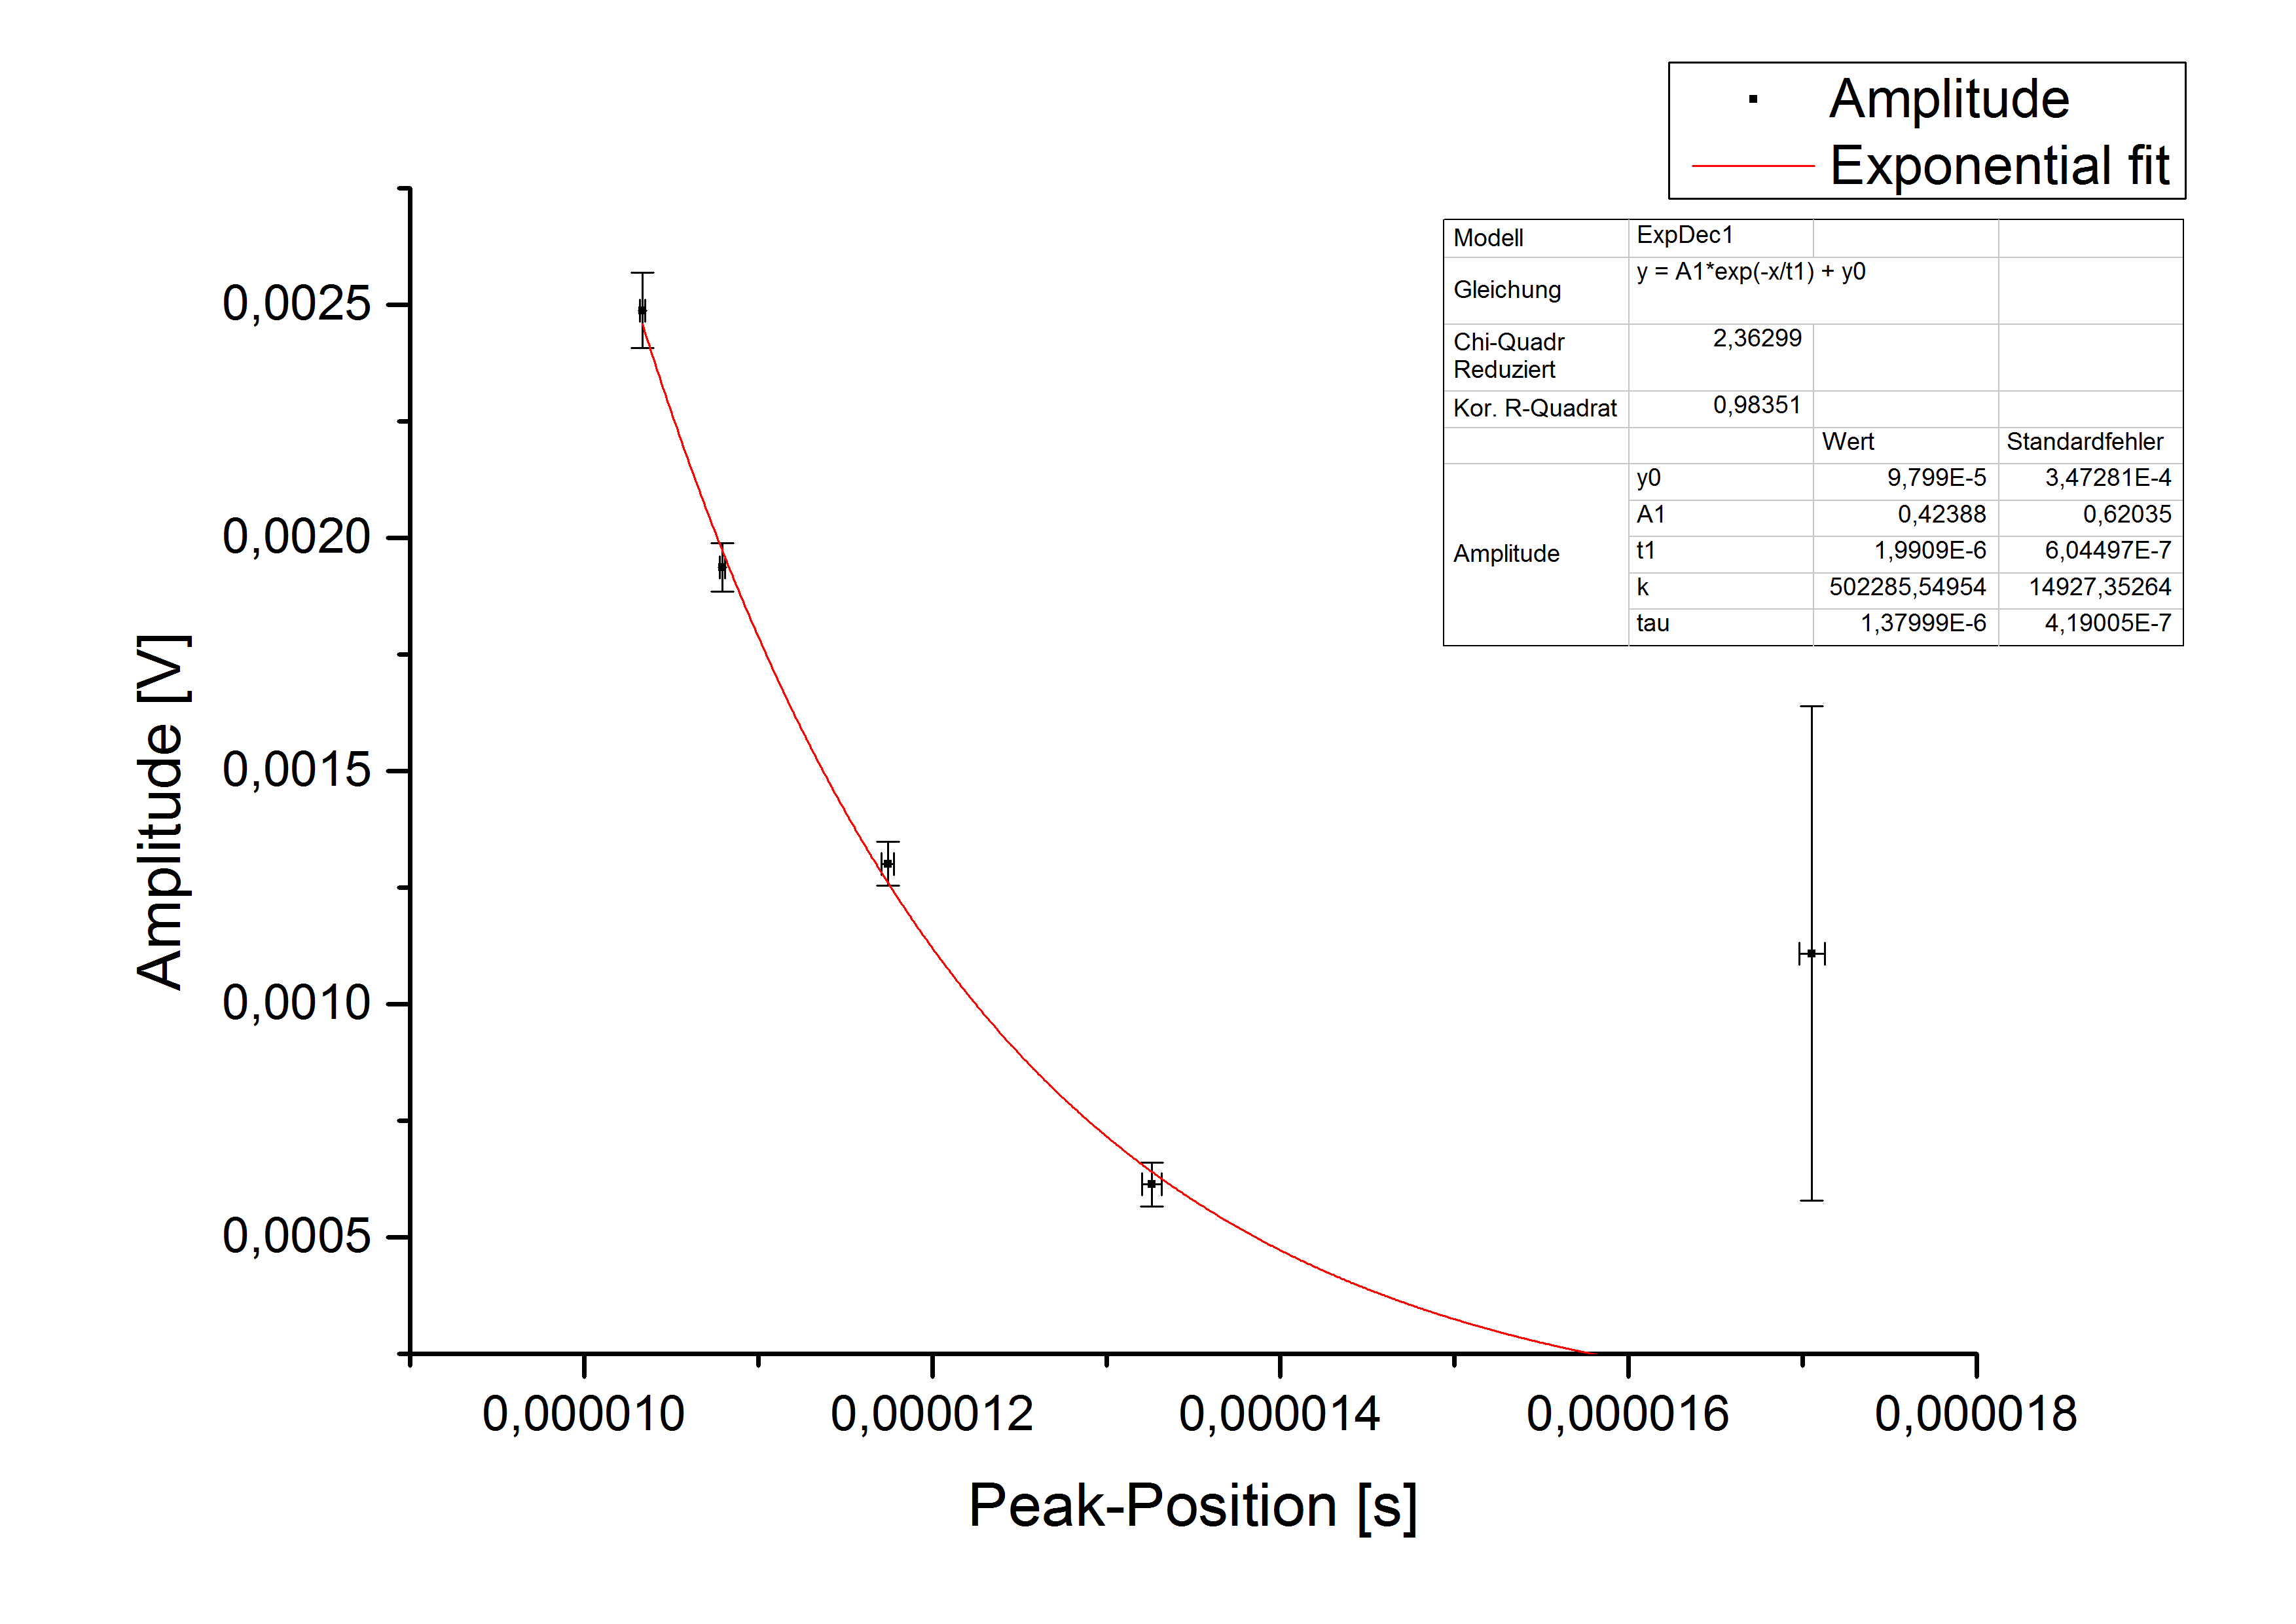
\includegraphics[scale=0.5]{Bilder/t2_2_tau}
\caption{Exponential decay fit of the amplitude, to get $\mathit{\tau}$. }
\label{fig:2tau}
\end{center}
\end{figure}\\
\newpage
The calculation of $\mathit{D_{n}}$ works the same way as in the first series.
\begin{figure}[h]
\begin{center}
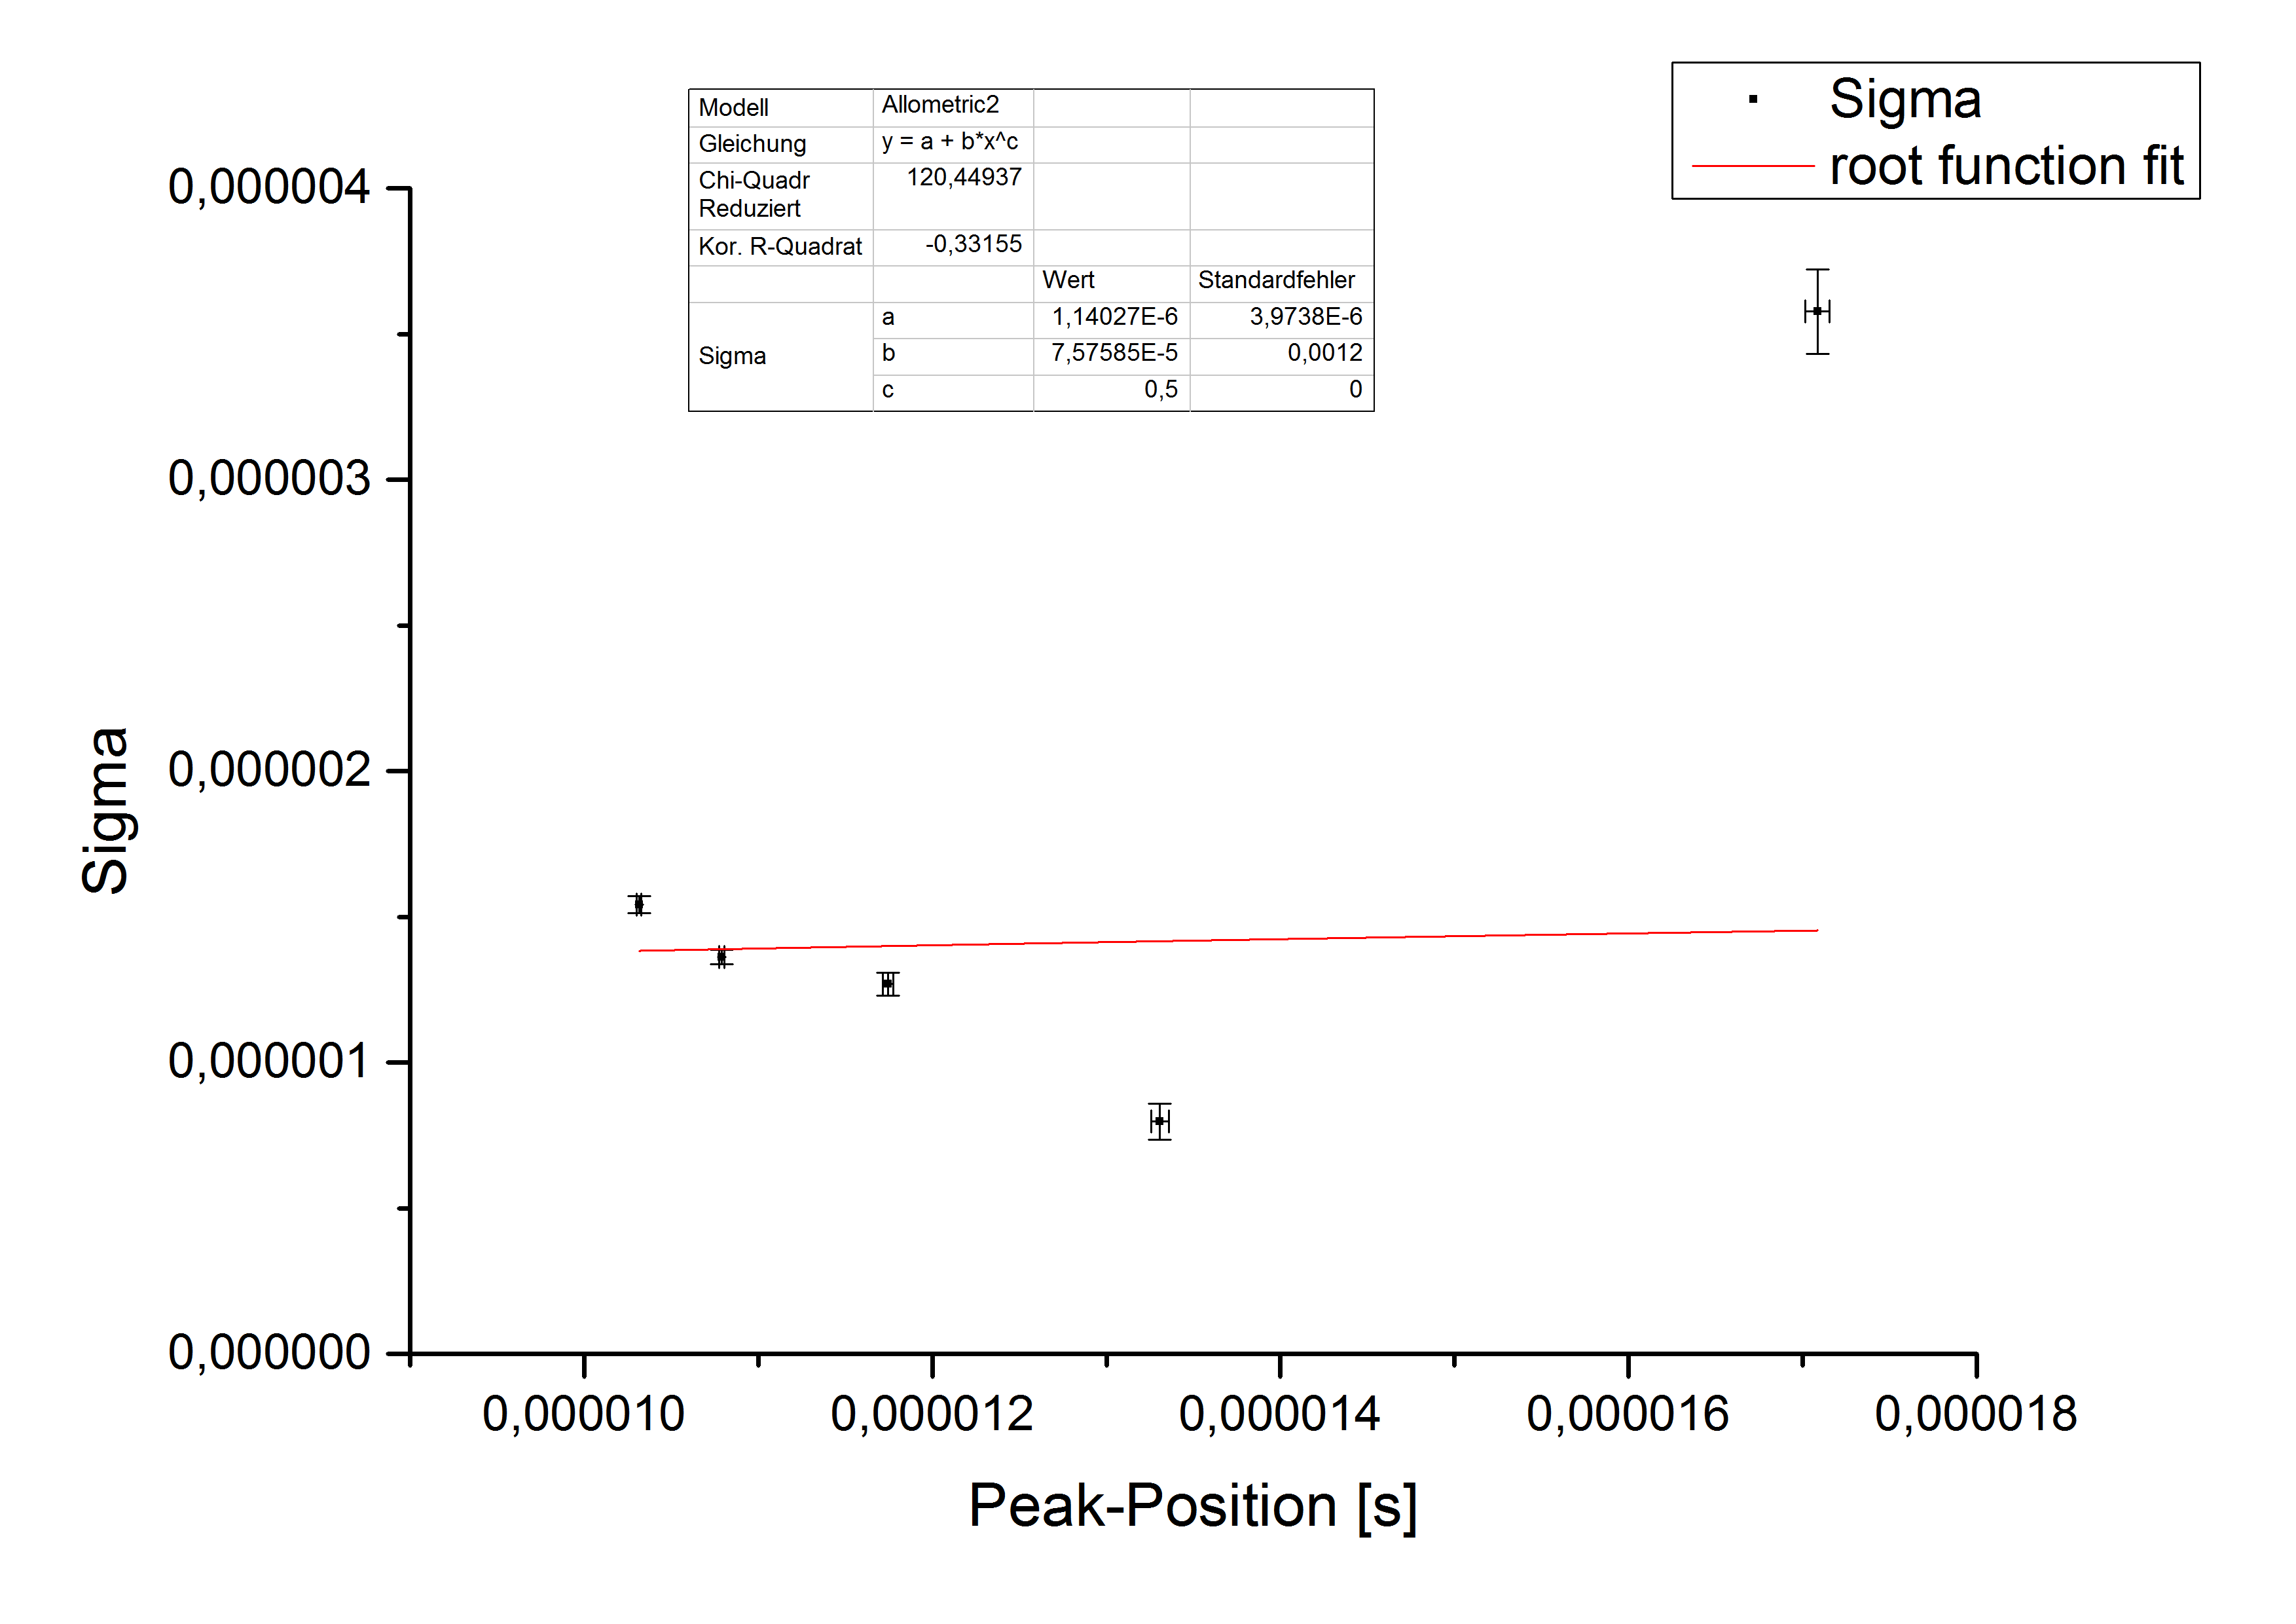
\includegraphics[scale=0.5]{Bilder/t2_2_sigma}
\caption{Exponential decay fit of the amplitude, to get $\mathit{\tau}$. }
\label{fig:2sigma}
\end{center}
\end{figure}\\
So our results from the second series of measurements is:\\

$\mathit{\mu_{n}=(2600\pm400)\frac{cm^{2}}{Vs}}$\\

$\mathit{\tau_{n}=(2.0\pm0.6)\cdot10^{-6}s}$\\

$\mathit{D_{e}=(0.3\pm9.1)\cdot10^{-8}\frac{mm^{2}}{s}}$

The literature values are the following:\\
\begin{center}
Mobility $\mu=3900 \frac{cm^2}{Vs}$\\
Mean lifetime $\tau=(45\pm 2)*10^{-6} s$\\
Diffusion constant $D_{n}=101 \frac{cm^2}{s}$
\end{center}
~\\
$\mu$ is in the same dimension of magnitude as the literature value. For $\tau$ and $D_{n}$, our results are far from their respective literature values. A possible explanation for this might be a contamination of the Ge-sample. Also, we did not take into account the errors on the oscilloscope. Still, we do not think these errors are what caused our bad results. As especially in the 2nd part of the experiment the signal decreased its width instead of increasing it, there has to be an issue about the oscilloscope causing a systematic error. 